% !TEX root = ../main.tex

\clearpage
\section{Appendix}
\appendix

\textblue{\textbf{Note to Reviewers:}} If accepted, the camera-ready version will link to a full version of the paper on eprint that will include the information in this appendix. We include it here for reference.

\section{CryptoKitty} \label{app:cryptokitty}

%Possibly remove this figure due to page limit
\begin{figure}[!htb]
\centering
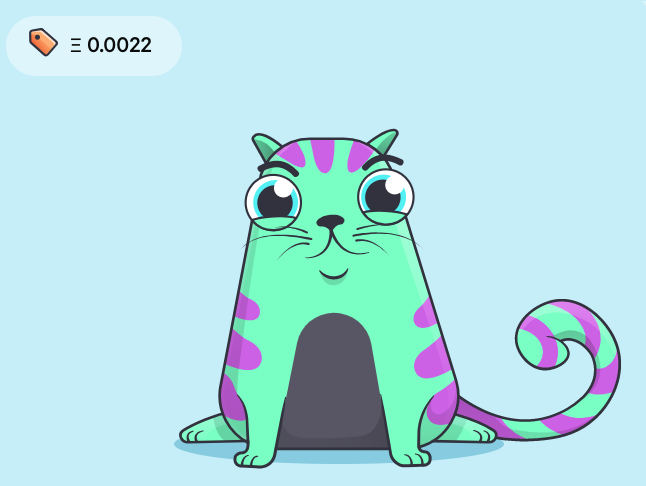
\includegraphics[width=0.3\linewidth]{figures/cryptokittie842912.png}
\caption{ Cryptokitty Number 842912 \label{fig:cryptokittie}}
\end{figure}

Figure~\ref{fig:cryptokittie} shows an example of a Cryptokitty.


\section{LocalEthereum} \label{app:localethereum}

%Possibly remove this code snippet due to page limit . don't forget to remove the refrence to it ^
\begin{lstlisting}[basicstyle=\scriptsize\ttfamily,caption={Code snippet from LocalEthereum smart contract. Values V,R and S are set by LocalEtherem to have a valid signature, also the tradeHash uses buyer and seller addresses, mitigating the possibility of front-running by a third party.},label={code:localethereum}]
    function createEscrow(bytes16 _tradeID, address _seller, address _buyer, uint256 _value, uint16 _fee,
					uint32 _paymentWindowInSeconds, uint32 _expiry, uint8 _v, bytes32 _r, bytes32 _s) 
        payable external {
        bytes32 _tradeHash = keccak256(abi.encodePacked(_tradeID, _seller, _buyer, _value, _fee));
	...
        // A signature (v, r and s) must come from localethereum to open an escrow
        bytes32 _invitationHash = keccak256(abi.encodePacked(
            _tradeHash,
            _paymentWindowInSeconds,
            _expiry
        )); 
\end{lstlisting}

Code~\ref{code:localethereum} shows a mitigation technique employed by LocalEthereum. \\



\section{Traditional Front-running Prevention Methods} \label{app:traditionalprevention}

There are debates in traditional markets regarding the fact that front-running is considered to be a form of insider trading which deemed to be illegal. Traditional methods to prevent front-running mainly involves after the fact investigation and legal action against the front-runners~\cite{FTFrontrunning18}. As mentioned in section~\ref{traditionalFrontrunning}, defining front-running and educating the employees were the first step taken to prevent such issues in traditional markets, however, front-running became less likely to happen mainly because of the high fine and lawsuits against firms who behaved in an unethical way. Other methods such as dark pools~\cite{zhu2014dark,buti2011diving} and sealed bids~\cite{radner1989sealed} were discussed and implemented in a variety of regulated trading systems. The traditional methods to prevent front-running does not apply to blockchain applications, as mainly they are based on central enforcement and limitations, also in case of blockchains the actors who are front-running could be anonymous and the fear of lawsuits would not apply. 


\section{Commit-and-Reveal} \label{app:cr}

\begin{figure}[!htb]
\centering
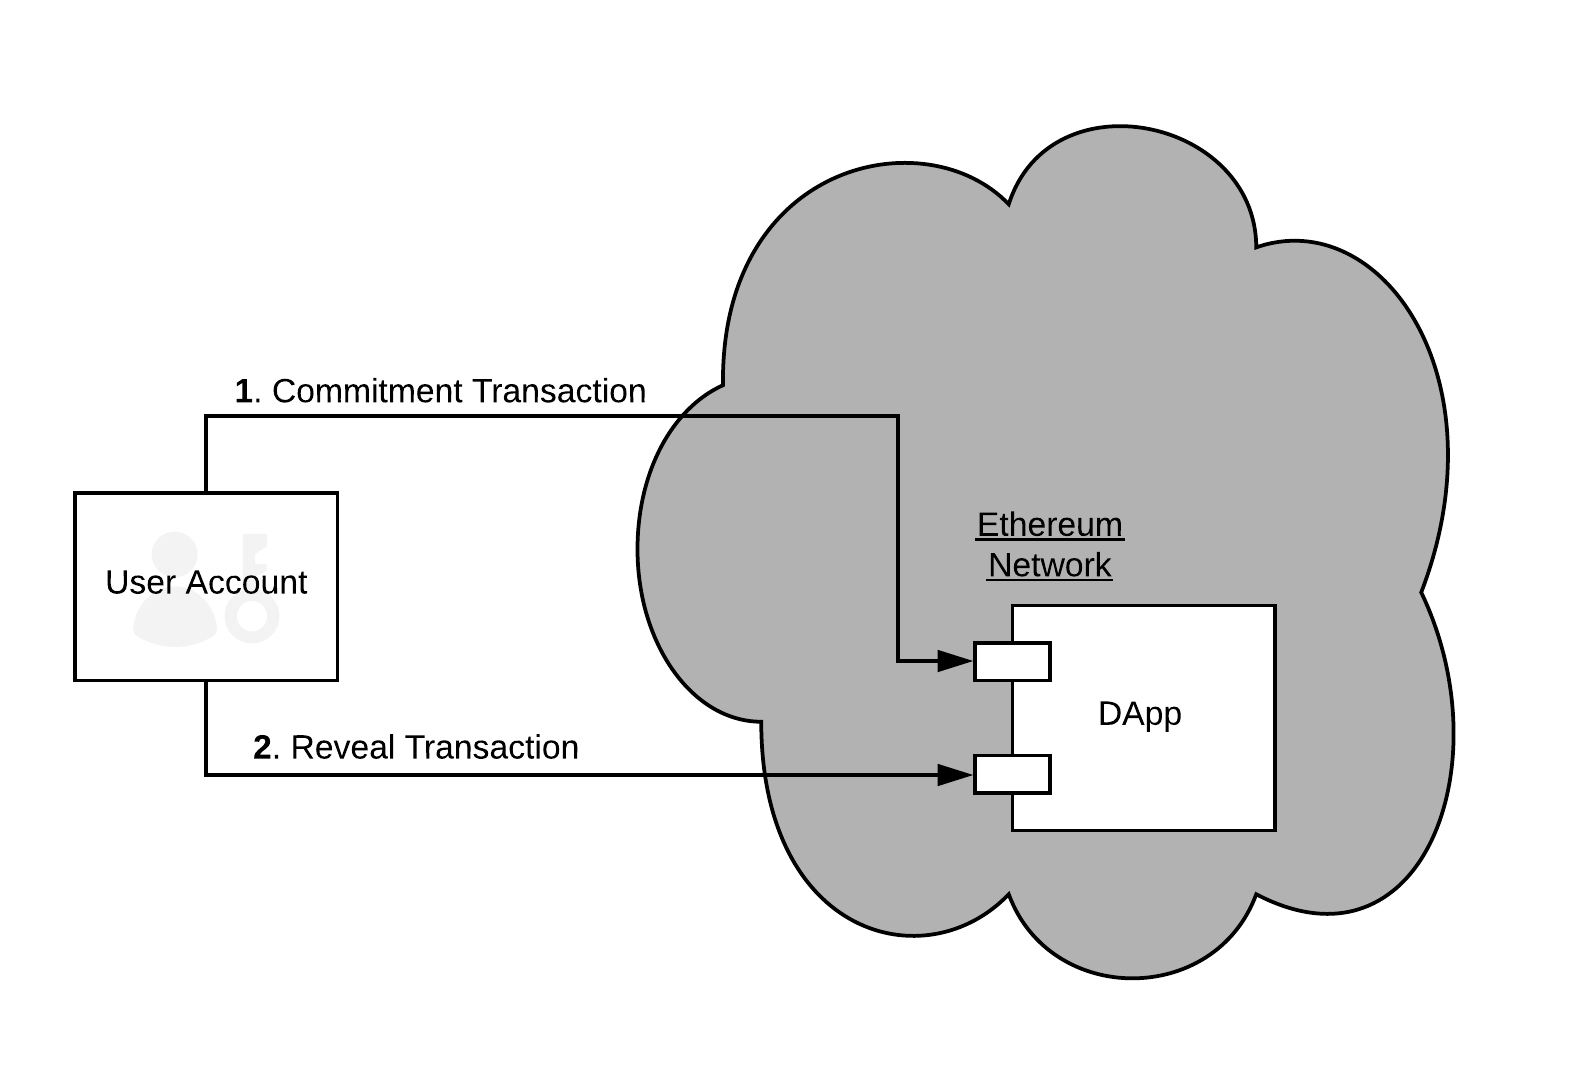
\includegraphics[width=0.5\linewidth]{figures/commit-reveal.png}
\caption{\scriptsize Commit and Reveal. User sends a commitment transaction with the hash of the data, After the commitment period is over, user sends her reveal transaction to the DApp revealing the information that matches the commitment. \label{fig:commitReveal}}
\end{figure}
%https://www.lucidchart.com/invitations/accept/3cd4c865-83d4-4c71-9a4a-f2e870f2db2c

Figure~\ref{fig:commitReveal} illustrates the commit/reveal approach.

%\section{Loop-ring}

%\paragraph{Design Decision \#3: Dual Authoring.} This scheme is proposed to solve the front-running issue within Loopring -- a decentralized exchange protocol proposed by Wang~\etal~\cite{wang2018loopring}. In the first version of this protocol, orders are grouped in \emph{ring orders} once they are sent by the users. After the required signatures are provided by the \textit{ring miner}, he sends the \emph{submitRing transaction} to the Loopring Smart Contract (LPSC) for verification and settlement (see Figure~\ref{fig:vulnerable_loopring}). While this transaction sits unconfirmed in the mempool, any front-runner can create a copy of this transaction with higher gasPrice and his address instead of the ring miner's address. Using the proposed \textit{dual authoring} solution in the new version of Loopring, regeneration of the \emph{submitRing transaction} is infeasible as the users have to sign the orders using their secondary private keys (auth-keys), which are only known to the ring miner and not other users (see Figure~\ref{fig:not_vulnerable_loopring}).
% Loopring protocol is proposed by Wang~\etal to build decentralized exchanges~\cite{wang2018loopring}. In this protocol, the orders are grouped in \emph{ring orders} immediately after they are sent by the users. Next, the required signatures are provided by a miner and owner of the order, see Figure~\ref{fig:vulnerable_loopring}. Eventually, the ring miner sends the \emph{submitRing transaction} to the Loopring Smart Contract (LPSC) for verification and settlement. While the \emph{submitRing transaction} sits unconfirmed in the mempool, any front-runner can create a copy of this transaction with his address instead of the ring miner's address and then sign the hash of the ring using his own private key. By paying a higher gasPrice, block miners choose the front-runner's transaction instead of the original \emph{submitRing transaction}. 
%To solve this issue, the new version of Loopring protocol uses the \emph{dual-authoring} scheme. This solution sets two levels of authorization for orders - one for settlement, and one for order matching. As it can be seen in Figure~\ref{fig:not_vulnerable_loopring}, each owner of an order generates a pair of public key (auth-address) and private key (auth-key), which are different from his address and its corresponding private key. These auth-keys are used to sign the hash of the ring and will further prevent anyone from regenerating the same \emph{submitRing transaction}. The reason is that the auth-keys are only known to the miner of the ring as they are not part of the on-chain transaction. Doing so, it is assured that (i) the orders are not modified because they are signed by the owner, (ii) no other miner can mine the ring because the miner's address is signed by the initial miner, and (iii) no user can front-run the \emph{submitRing transaction} because other users do not have access to the auth-keys and hence are not able to generate new transactions with auth-keys signatures on them.

%\begin{figure}[t]
%\centering
%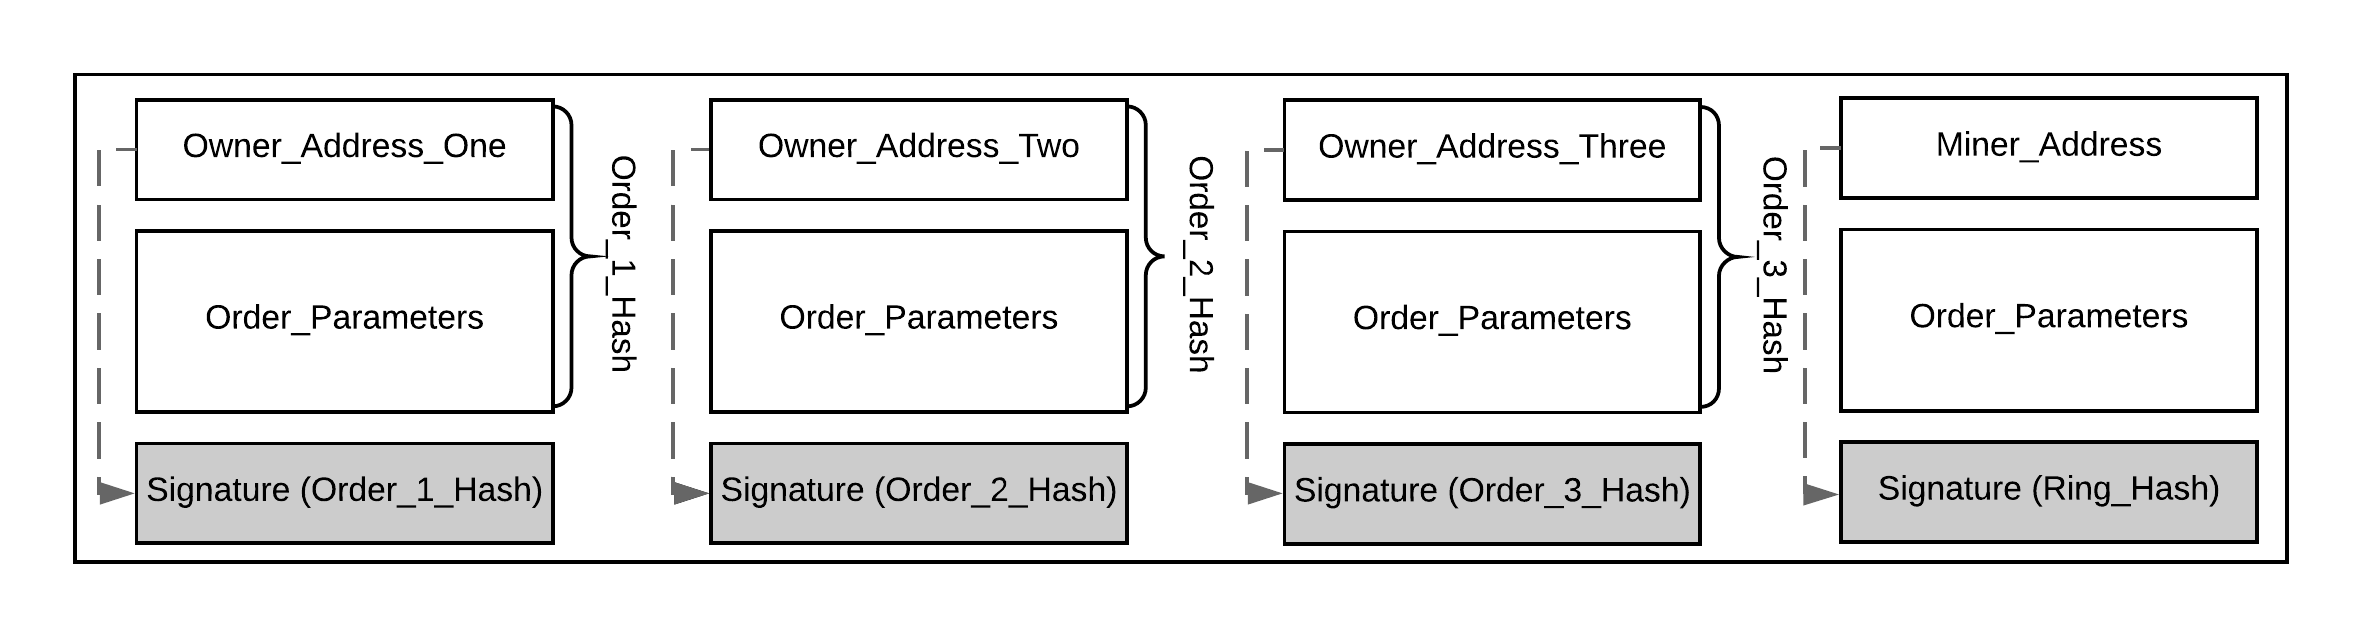
\includegraphics[width=0.9\linewidth]{figures/Vulnerable_Loopring.png}
%\caption{ \emph{submitRing} Transaction in the old version of the Loopring protocol. Any user can regenerate this transaction by replacing the miner's address with his address and signing the hash of the ring using his private key. \label{fig:vulnerable_loopring}}
%\end{figure}
%https://www.lucidchart.com/invitations/accept/33d38ce9-4660-4743-806d-45c72f7e8393
%\begin{figure}[t]
%\centering
%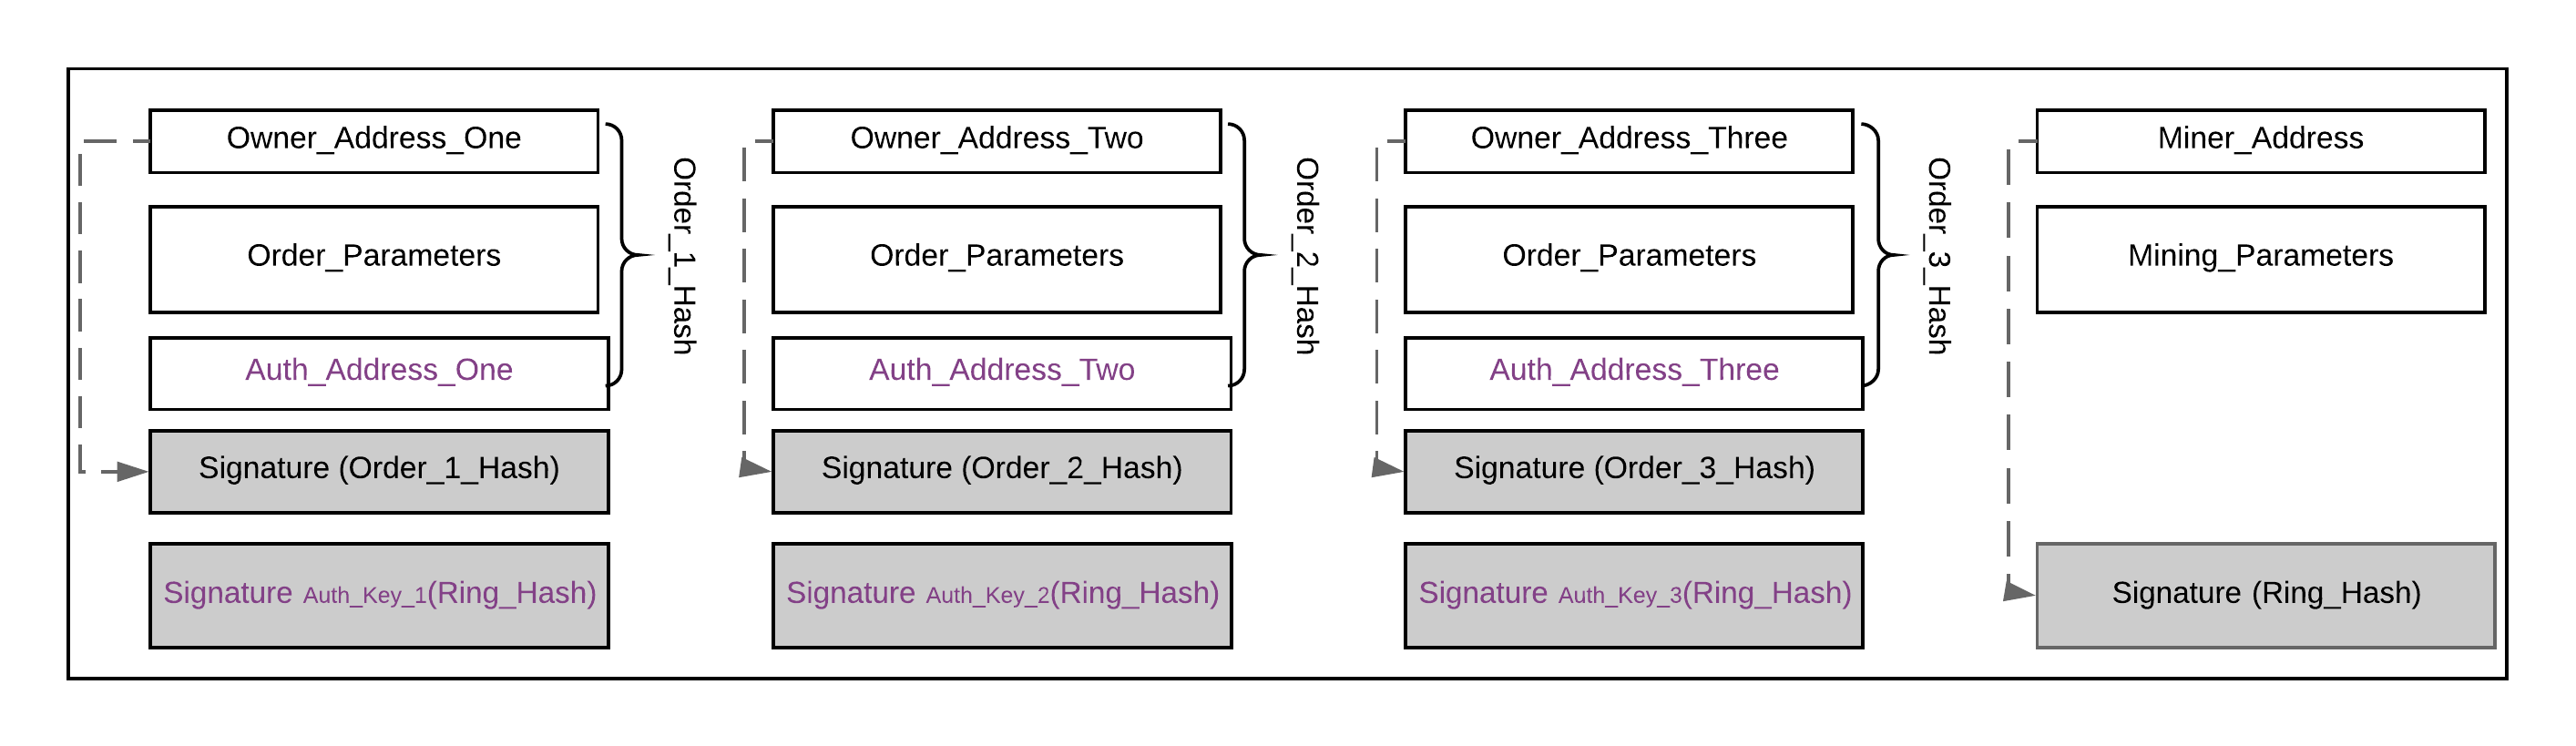
\includegraphics[width=0.7\linewidth]{figures/Dual_Authoring_Loopring.png}
%\caption{ \emph{submitRing} Transaction in the new version of the Loopring protocol. Other users cannot regenerate this transaction as they do not access auth-keys and hence are not able to create the signatures. \label{fig:not_vulnerable_loopring}}
%\end{figure}
%https://www.lucidchart.com/invitations/accept/8dee869c-482c-433f-a901-8d041a1dc526

%The first solution was to prevent front-running, but then it was attacked so they updated the solution. this new solution also could be attacked. 

